\documentclass[15pt]{article}
\usepackage[utf8]{inputenc}
\usepackage[spanish]{babel}
\usepackage{amsmath}
\usepackage{amsthm}
\usepackage{amssymb}
\usepackage{fancyhdr}
\usepackage[margin=0.9in]{geometry}
\usepackage{listings}
\usepackage{listingsutf8}
\usepackage{algorithm}
\usepackage{url}
\usepackage{graphicx}
\usepackage{minted}

\usepackage[export]{adjustbox}

\graphicspath{./}
\pagestyle{fancy}
\lhead{Práctica 6: Balanceador de carga}
\rfoot{\thepage}
\lfoot{ESCOM-IPN}
\renewcommand{\footrulewidth}{0.5pt}
\bibliographystyle{IEEEtran}

%opening
\title{Práctica 6: Balanceador de carga}
\author{3CM7}
\date{3 de diciembre de 2018}

\begin{document}
	
	\begin{titlepage}
		\begin{center}
			
			% Upper part of the page. The '~' is needed because \\
			% only works if a paragraph has started.
			
			\noindent
			\begin{minipage}{0.5\textwidth}
				\begin{flushleft} \large
					
\includegraphics[width=0.3\textwidth]{ipn.png}
				\end{flushleft}
			\end{minipage}%
			\begin{minipage}{0.55\textwidth}
				\begin{flushright} \large
					
\includegraphics[width=0.7\textwidth]{escom.png}
				\end{flushright}
			\end{minipage}
			
			\textsc{\LARGE Instituto Politécnico Nacional}\\[0.5cm]
			
			\textsc{\Large Escuela Superior de Cómputo}\\[1cm]
			
			% Title
			
			{ \huge Práctica 6: Balanceador de carga \\[1cm] }
			
			{ \Large Unidad de aprendizaje: Aplicaciones para comunicaciones en red} \\[1cm]
			
			{ \Large Grupo: 3CM7 } \\[1cm]
			
			\noindent
			\begin{minipage}{0.5\textwidth}
				\begin{flushleft} \large
					\emph{Alumnos:}\\
					\begin{itemize}\setlength\itemsep{0em}
						\item Ontiveros Salazar Alan Enrique
						\item Sánchez Valencia Sergio Gabriel
					\end{itemize}
				\end{flushleft}
			\end{minipage}%
			\begin{minipage}{0.5\textwidth}
				\begin{flushright} \large
					\emph{Profesor:} \\
					Moreno Cervantes Axel Ernesto
				\end{flushright}
			\end{minipage}
			
			\vfill
			
			% Bottom of the page
			{\large 3 de diciembre de 2018}
		\end{center}
	\end{titlepage}

	\maketitle
	
	\section{Marco teórico}
		\subsection{Balanceador de carga}
		Es una técnica para distribuir o compartir cargas de trabajo a través de múltiples recursos de cómputo, tales como computadoras, clústers, enlaces de red, unidades de proceso o discos duros. Su objetivo es optimizar el uso de recursos, maximizar el rendimiento y minimizar el tiempo de respuesta, evitando la sobrecarga de un único recurso.
		
		El uso de múltiples componentes con balance de carga en lugar de uno solo puede incrementar la confiabilidad y la disponibilidad, a costa de una mayor redundancia. El balance de carga se lleva a cabo con software o hardware dedicado.
		
		Internamente, está basado en algún algoritmo que divide de la manera más equitativa posible la carga de trabajo, para evitar los famosos cuellos de botella.
		
		\begin{figure}[H]
			\centering
			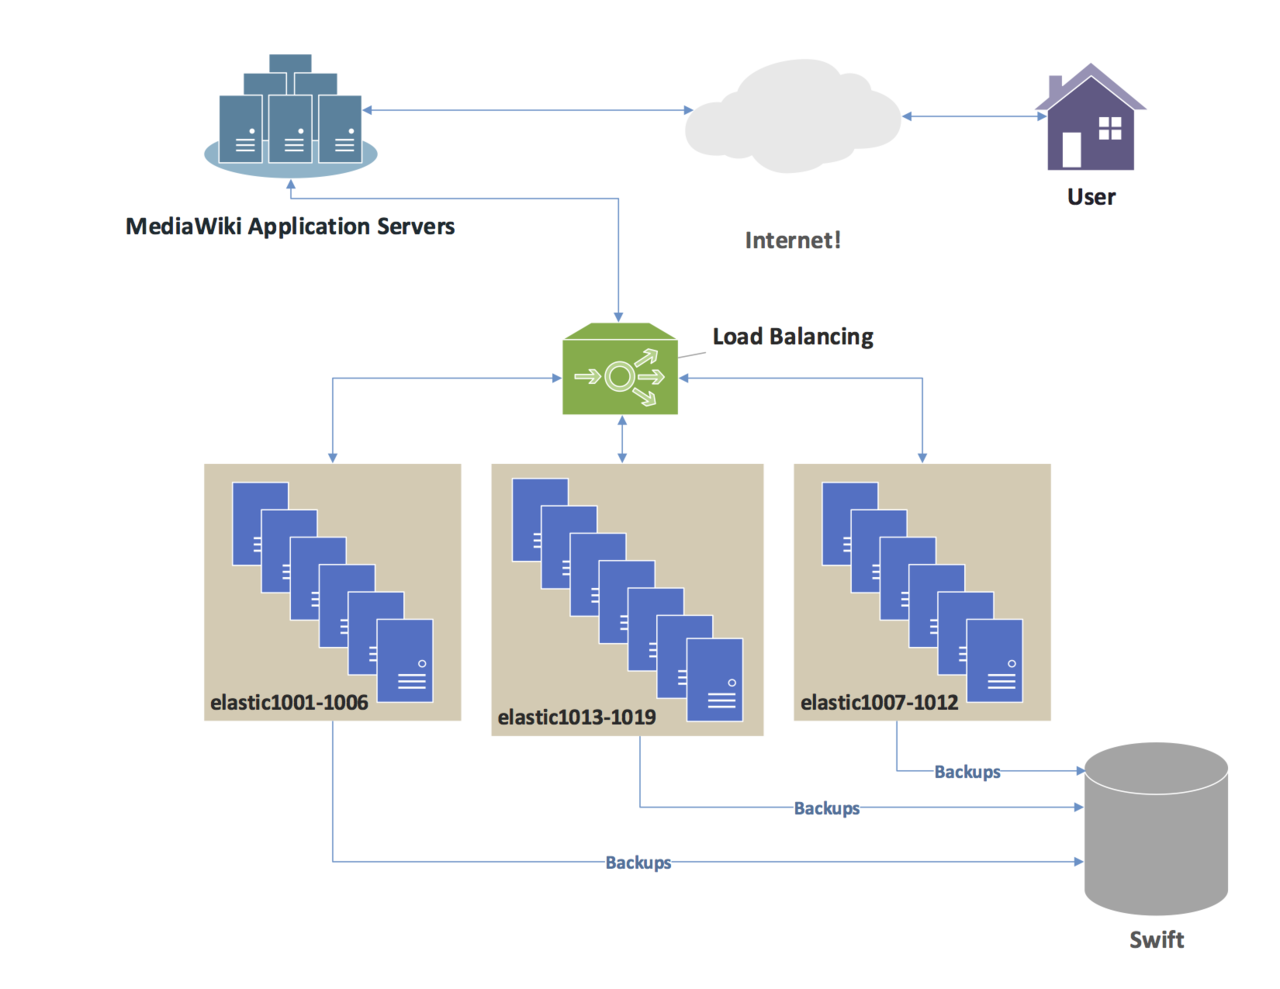
\includegraphics[scale=0.6]{load.png}
			\caption{Diagrama básico de un balanceador de carga}
		\end{figure}
	
		\subsection{Round-robin}
		Es un algoritmo de planificación en computación. Consiste en asignarle a cada proceso unidades de tiempo iguales (quantums) en un orden circular, manejando todos los procesos sin prioridad. Es un algoritmo simple y fácil de implementar.
		
		Distribuye todo de manera equitativa y en un orden racional, normalmente comenzando por el primer elemento de la lista hasta llegar al último y empezando de nuevo desde el primer elemento.
	
	\section{Desarrollo}
		En esta práctica usaremos el servidor HTTP que hicimos en la práctica 4, solo que esta vez lo correremos simultáneamente en distintos puertos (del \texttt{5678} al \texttt{5681}) para tener cuatro disponibles. Haremos un nuevo servidor en el puerto \texttt{1234} que actuará de forma similar a un proxy: recibirá todas las solicitudes HTTP que le lleguen y las repartirá a un puerto de los disponibles, luego esperará su respuesta mediante un socket bloqueante y la regresará al cliente que la solicitó mediante el socket no bloqueante.
		
		Internamente llevaremos una variable que nos dirá la posición del servidor actual, de tal forma que se estará incrementando cada vez que llegue un nuevo cliente, y regresando a 0 si ya usamos todos los servidores (esto se logra de manera muy sencilla con el operador módulo), algo parecido a una cola circular. Así logramos que la repartición de la carga sea lo más igual posible entre todos los servidores disponibles.
	
	\clearpage
	\section{Pruebas}
		Corremos los cuatro servidores:
		\begin{figure}[H]
			\centering
			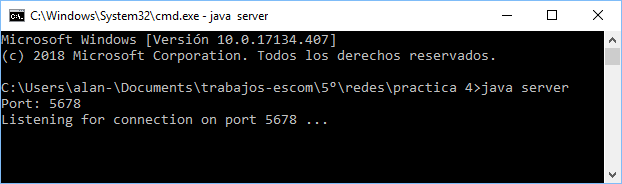
\includegraphics[scale=0.9]{s1.png}
		\end{figure}
		\begin{figure}[H]
			\centering
			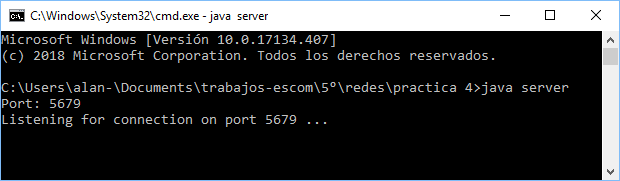
\includegraphics[scale=0.9]{s2.png}
		\end{figure}
		\begin{figure}[H]
			\centering
			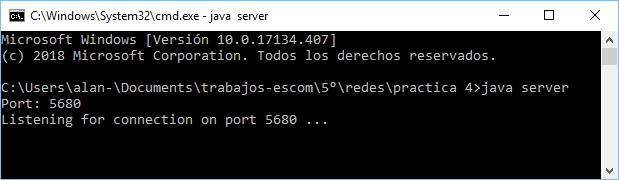
\includegraphics[scale=0.9]{s3.png}
		\end{figure}
		\begin{figure}[H]
			\centering
			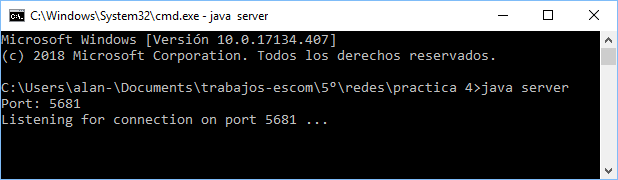
\includegraphics[scale=0.9]{s4.png}
		\end{figure}
		
		\clearpage
		Corremos el balanceador de carga:
		\begin{figure}[H]
			\centering
			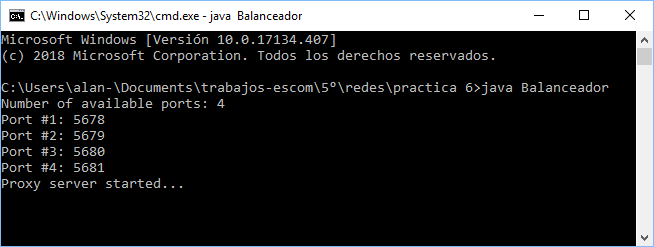
\includegraphics[scale=0.9]{bal.png}
		\end{figure}
		
		\clearpage
		Realizamos algunas solicitudes desde el navegador:
		\begin{figure}[H]
			\centering
			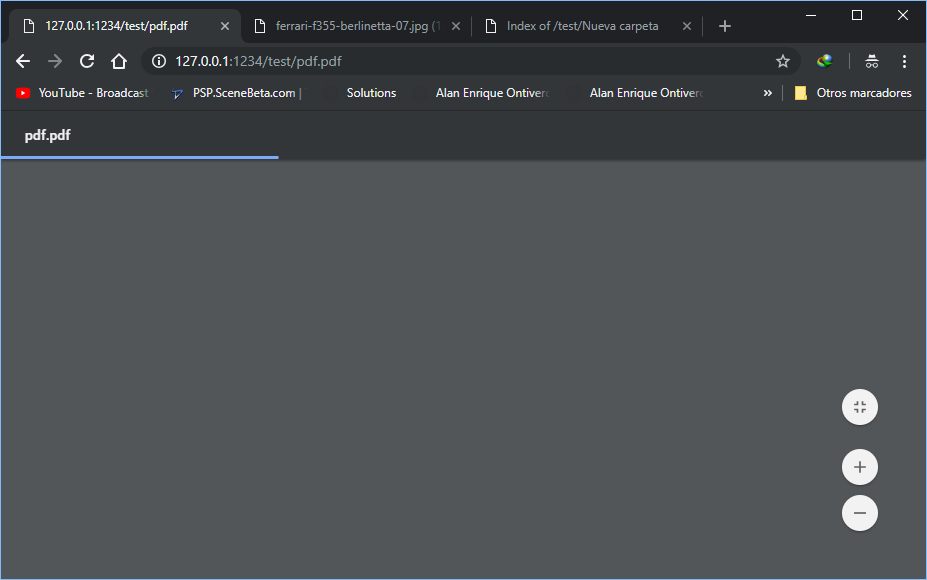
\includegraphics[scale=0.75]{requests.png}
		\end{figure}
	
		Y vemos cómo éstas se repartieron entre los cuatro servidores:
		\begin{figure}[H]
			\centering
			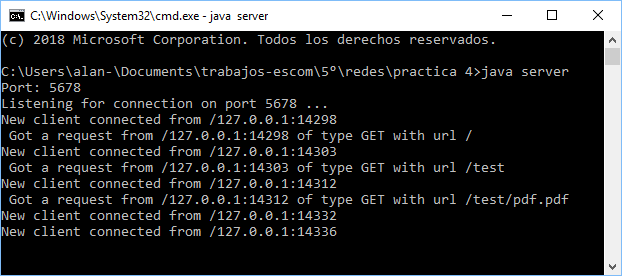
\includegraphics[scale=0.9]{r1.png}
		\end{figure}
		\begin{figure}[H]
			\centering
			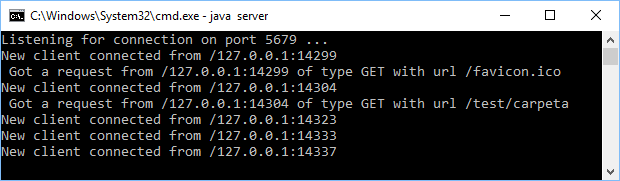
\includegraphics[scale=0.9]{r2.png}
		\end{figure}
		\begin{figure}[H]
			\centering
			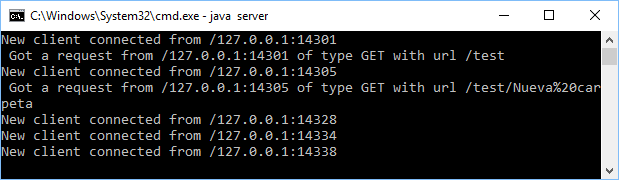
\includegraphics[scale=0.9]{r3.png}
		\end{figure}
		\begin{figure}[H]
			\centering
			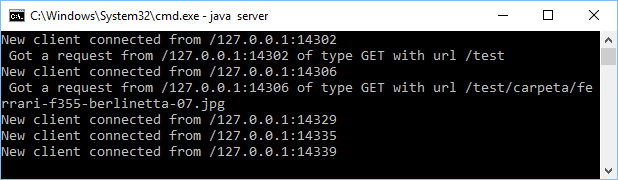
\includegraphics[scale=0.9]{r4.png}
		\end{figure}
		
	
	\clearpage
	\section{Conclusiones}
		Al usar sockets no bloqueantes evitamos la creación de un hilo por cada cliente que llegue; en lugar de eso Java implementa la técnica de los selectores, que nos dicen los eventos con los que nosotros podemos interactuar (lectura, escritura, nueva conexión, etc.), y justo en el momento que los necesitamos. De esta manera solo necesitamos crear un hilo, optimizando memoria y tiempo de procesamiento.
	
	
\end{document}